\chapter{Konzept}
\label{ch:chapter04}
In diesem Kapitel wird darauf eingegangen wie Vorgegangen wurde, um verschiedene Konzepte zu entwickeln.
Dabei werden die vorher erwähnten Befragungen (\ref{ch:Recherche}) verwendet, um eine Lösung für die individuellen Probleme zu entwickeln.
Zudem wird betrachtet der Stand der Technik betrachtet sowie einen Vergleich mit den Datenbankstrukturen gezogen.
Dies wird getan, da diese eine ähnliche Struktur wie die Profile und Berechtigungen.
Anschließend werden die Probleme aus den Befragungen quantifiziert, um daraus dann die verschiedenen Konzepte zu entwickeln.


\section{Konzeptentwicklung}
\label{sec:chapter04:Konzeptentwicklung}

\subsection{Stand der Technik}
\label{sec:chapter04:Stand}
In der Welt von Cloud Computing wird \ac{IAM} als Sicherheitsmaßnahme verwendet.
Dabei wird mittels \ac{IAM} die Identität und der Zugriff reguliert.
\ac{IAM} kann daher in die folgende fünf Punkte gegliedert werden.
\newline
\newline
1. Authentifizierung der Person
\newline
Dabei überprüft, ob die Person auch wirklich, die ist als welche diese sich ausgibt.
Hierfür gibt es verschiedene Methoden, um dies sicherzustellen.
Nutzername mit ein Passwort ist die gängigste Methoden, um dies zu tun, welche von den meisten Webseiten und Computern verwendet wird.
Um die Authentifizierung sicherer zu gestalten werden mehrere Faktoren berücksichtigt, um eine Person zu identifizieren.
Dies kann zum Beispiel durch einen Fingerabdruck stattfinden. \cite{IamIEEE} (S.1482)
\newline
\newline
2. Berechtigungsvergabe
\newline
Es beschäftigt sich damit, welche Berechtigungen der Nutzer bekommt.
Dies wird mittels Autorisierungsrichtlinien gesichert, damit die Nutzer nur Zugriff auf die Ressourcen und Dienste haben, welche diese benötigen.
Das wird mit hilfe von Profilen erreicht, welche von der Organisation zugewissen werden. \cite{IamIEEE} (S.1482)
\newline
\newline
3. Identitätsvergabe
\newline
Identitätsvergabe sorgt dafür, dass der Nutzer eine digitale ID oder Account erhält.
Wenn ein Mitarbeiter bei einem Unternehmen arbeit, erhält dieser eine digitale Identität, um auf die Ressourcen des Unternehmen zu greifen zu können.
Dabei ist auch wichtig, dass der Mitarbeiter diese digitale Identität wieder verliert, wenn dieser das Unternehmen verlässt oder an einer anderen Stelle im Unternehmen arbeitet und nicht mehr seine alte digitale Identität benötigt.
\newline
\newline
4. Föderierte Identität
\newline
Dabei handelt es sich darum, dass die digitalen Identitäten über verschiedene Anwendungen und Organisationen gültig sind.
Dadurch werden die Informationen der digitalen Identität gespeichert.
Dies hat den Vorteil, dass der Nutzer sich nur einmal anmelden muss, um auf sämtliche seiner Ressourcen zugreifen zu können.
Dabei werden Protokolle wie SAML, OAuth oder OpenID verwendet.
Die Folge dadurch ist, dass der Nutzer sich nicht mehrere Passwörter sowie Accounts merken muss. \cite{IamIEEE} (S.1482)
\newline
\newline
5. Compliance Verwaltung
\newline
Die Compliance Verwaltung überprüft die Authentifizierung- und Zugriffaufzeichnungen, um sicher zustellen, dass die Richlinien und Sicherheitsstandards eingehalten wurden.
Diese Überprüfung ist notwendig für effektive Zugriffregeln.
Zudem werden diese für Audits benötigt. \cite{IamIEEE} (S.1482)
\newline
\newline
\begin{figure}[h!]
 \centering
 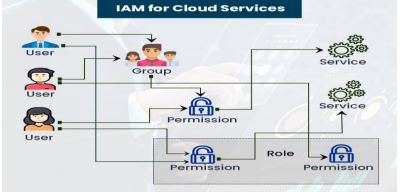
\includegraphics[width=1\textwidth]{gfx/Picture/IAMISH.PNG}
 \caption{IAM für Cloud Dienste \cite{Moha19} (Seite 3)}
 \label{fig:IMAISH}
\end{figure}
Dies ist ein Beispiel wie die oben genannten Punkte umgesetzt werden können.
Dabei haben die Accounts der Personen entweder direkte Berechtigung oder diese werden mittels Gruppen verteilt.
Sobald der Account die Berechtigung hat, kann dieser auf die dahinter steckende Ressource zugreifen.
Die Berechtigungen können dabei auch mittels Profile zusammengefasst werden.
\newline
Dabei kann dies auch verschiedenen Wegen umgesetzt werden, da die selbe Lösung für gewisse Fälle nicht funktioniert.
Zum Beispiel die Quelle \cite{Cal17}(S.208) beschreibt das Problem wie die United States of America am besten mit ihren Verbündeten kooperieren soll.
Da es dabei um sensitive Informationen handelt, welche an verschiedenen Partnern vermittelt werden, muss der Zugriff reguliert werden.
Besonders haben die verschiedenen Ländern verschiedene Gesetzte, worauf auch geachtet werden muss. 
Deswegen gibt es nicht die eine Lösung, um die Herausforderung zu lösen. \cite{Cal17} (S.208)


\subsection{Vergleich mit Datenbanken}
\label{sec:chapter04:DB}
Die Helvetia verwendet zum Speichern der Informationen für die Berechtigungsstruktur so genannte HV-Tabellen.
Bei diesen HV-Tabellen handelt es sich dabei, um DB2-Tabellen.
Zudem besteht zwischen eine Ähnlichkeit zwischen dem Nutzer und Profil in der Berechtigungsstruktur zu dem Account und Gruppe in Datenbanken.
Deswegen wird betrachtet, wie der Standard mit Accounts und Gruppen innerhalb von Datenbanken ist.
\newline
Berechtigungen für Rollen wird mittels GRANT...ON...TO...[GRANT OPTION] vergeben.
Dabei wird die spezifische Berechtigungen, zum Beispiel eine View und Account oder Gruppen angegeben.
Zudem kann auch hinzugefügt werden, ob die Rolle die Berechtigung hat anderen Accounts die Berechtigungen zu geben.\cite{Ram09} (S.474-475)
\newline
Wenn man sich zum Beispiel das Bild (\ref{fig:Berch}) ansieht könnte zum Beispiel der Befehl wie folgt aussehen:
\newline
\newline
GRANT UPDATE ON PKU00 TO L895.
\newline
\newline
Das würde zum Beispiel bedeuten, dass der Nutzer L895 die Bearbeitungsberechtigung für die Ressource PKU00 erhalten hat.
Dabei kommt auch die Frage, was man eher verwenden sollte.
Indviduelle Berechtigungsvergabe oder über Gruppenvergabe für die Accounts.
Microsoft hat folgendes als Best Practise definiert:
\newline
\newline
\textit{"`To simplify administration, create groups and assign each group permission to functional areas and model objects.
You can then add and remove users from the groups without accessing the Master Data Manager UI.
\newline
\newline
Do not assign additional permissions to an individual user, and do not include a user in multiple groups that have access to Master Data Manager. In addition, do not use hierarchy member permissions unless you want a group to have limited access to specific members."'} \cite{Micro}
\newline
\newline
Micrsoft gibt an, dass man Gruppen erstellen, die individuellen Nutzer keine zusätzlichen Berechtigungen bekommen sollen und nicht in mehreren Gruppen sein soll, die Zugriff auf den Master Data Manager haben.
IBM gibt eine ähnlich Best Practise an, dass Angestellte in einem Unternehmen mittels Gruppen organisiert werden sollten. \cite{IBMGroup}

\section{Herausforderung und Anforderungen}
\label{sec:chapter04:Herausforderung}
Bei der Rechereche (\ref{ch:Recherche}) sind verschiedene Herausforderungen und Anforderungen aufgetreten.
Um qualitativ ein Konzept zu entwickeln zu können, müssen diese Herausforderungen und Anforderungen aufgelistet and analysiert werden.
\begin{itemize}
	\item Performance der Tabellen erhöhen (effizientere Verifizierung der Mitarbeiter)
	\item Übersichtlicher gestalten
	\item Rekursive Beziehungen verhindern
	\item Hierarchie verringern
	\item \ac{K/W}
\end{itemize}
Um diese zu quantifizieren zu können wird eine Prioritätsanalyse (\ref{fig:Prio}) verwendet, um festzustellen, wie die Priorität für die Konzepte sein muss. \cite{BdIufH}
Bei der Prioritätsanalyse wurde sich für ein vier Punktesystem entschieden.
\newline
Im Vergleich zwischen Performance und Übersichtlich wurde Performace drei Punkte gegeben und übersichlich hat nur einen Punkt erhalten, da die Performance einer der Grundanforderungen ist, weswegen die Berechtigungsstruktur geändert werden soll.
Die Übersichtlichkeit dazu im Vergleich ist weniger wichtig.
Performance und Rekursive haben jeweils zwei Punkte bekommen, da eine performante Struktur keine rekursiven Beziehungen enthält.
Die Performance hat vier Punkte zur Hierarchie null Punkten erhalten, weil die Verringerung der Hierarchie kaum einen Einfluss auf die jährliche Rezertifizierung hat.
\ac{K/W} sowie Performance haben zwei Punkte bekommen.
Dies liegt daran, dass neben der Performance die \ac{K/W} elementar sind, da ein Struktur, die sich kaum warten lässt mehr Ressourcen kosten wird in der Zukunft.
Zwischen Übersichtlich und Rekursive wurde Rekursive drei Punkte gegeben und Übersichlich nur einen, weil rekursive Strukturen unübersichlicher sind und es daher wichtiger ist, dass es keine gibt, damit diese übersichtlich wird.
Übersichtlich und Hierarchie haben beide zwei Punkte erhalten, da beide eine gleiche Rolle zur Lesbarkeit der Struktur spielen.
Übersichtlich sowie Rekursive und Hierarchie bekommen einen Punkt im Vergleich zu \ac{K/W}, weil dieser Punkt langfristig eine wichtige Rolle ist und die anderen drei Punkte sollten kein Problem sein, sofern sich an die Konventionen gehalten werden, damit die Struktur wartbar bleibt.
Rekursive bekommt vier Punkte zu Hierarchie null Punkten, da eine rekursive Beziehung die Hierarchie automatisch unendlich macht.
\newline
\newline
Wenn man dies dann auswertet, bekommt Performance einen Gewichtsfaktor von 27,5\%, Übersichlich 12,5\%, Rekursive 25\%, Hierarchie 7,5\% und \ac{K/W} 27,5\%.
Dadurch sieht die Rangfolge wie folgt aus:
\begin{enumerate}
	\item Performance | \ac{K/W}
	\item Rekursive
	\item Übersichlich
	\item Hierarchie
\end{enumerate}
Anhand dieser Reihenfolge werden die folgenden Konzepte entwickelt.
\begin{figure}[h!]
 \centering
 \includegraphics[width=1\textwidth]{gfx/Picture/Prioritatätsanalyse.PNG}
 \caption{Prioritatätsanalyse der Kriterien}
 \label{fig:Prio}
\end{figure}

\section{Konzept Struktur}
\label{sec:chapter04:Struktur}
Das erste Konzept Struktur ist wie folgt aufgebaut.
\begin{figure}[h!]
 \centering
 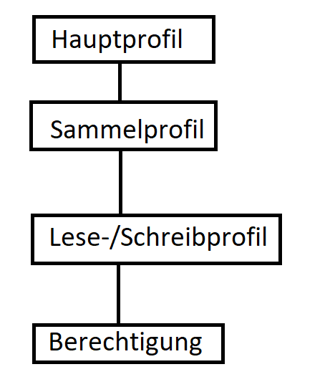
\includegraphics[width=0.75\textwidth]{gfx/Picture/Hierarchie.PNG}
 \caption{Hierarchie für Konzept Struktur}
 \label{fig:Struktur}
\end{figure}
Wie man in der Graphik (\ref{fig:Teil}) erkennen kann, gibt es bei der aktuellen Berechtigungsstruktur keine Struktur.
Um dementsprechend die genannten Problem zu beheben wurde die neue Struktur (\ref{fig:Struktur}) entwickelt.
Um die \ac{K/W} wurden die folgenden Konvention für dieses Konzept entwickelt.
Profile enthalten nur noch Profile oder Berechtigungen.
Die Berechtigungsstruktur soll nur noch ein Hierarchietiefe von maximal vier haben.
Die erste Hierarchiestufe enthält das Standardprofil, welche dem Nutzer gegeben wird.
Die zweite Hierarchiestufe enthält die jeweiligen Sammellese- und Sammelschreibeprofile, die jeweils in ihre Fachbereiche getrennt sind.
Die dritte Hierarchiestufe enthält die individuellen Lese- und Schreibprofile.
Die vierte Stufe enthält die Berechtigungen.
Manche der bestehenden Profile beinhalten aktuell was zukünftig Hauptprofile wären.
In solchen Fällen würde diese Profile zu Hauptprofilen werden und vom vorherigen Hauptprofil separiert werden.
Manche Fachbereiche haben aufzählende Profile (\ref{fig:Profile}).
Diese Profile sollen nur noch über die Berechtigungen für den eigenen Vorgang enhalten, sodass ein Privas Profil nur Privas Berechtigungen enthält.
Die Berechtigung die verloren gehen würden eigene Profile bekommen und würden über ein anderes Sammelprofil dem Hauptprofil hinzugefügt werden.
Sollte ein Nutzer weitere Berechtigungen benötigen, würden diese über ein anderes Hauptprofil, welches am ehesten für die Aufgabe passt, zugeordnet.
Wenn ein Account reaktiviert wird, muss dieser rezertifiziert werden.
\newline
Diese Konventionen sollen verhindern, dass die Struktur weiter wächst und das man ohne Problem feststellen kann, was für Berechtigungen ein Profil man hat.
Zudem hat es Vorteil, dass rekursive Beziehung sowie redundante Berechtigungsvergabe nicht möglich sind, da die Profile nur noch Profile oder Berechtigungen enthalten, die nicht mehr auf sich gegenseitig zeigen sollen sondern höchstens sammeln soll.
Dadurch soll auch die Übersichlichkeit verbessert und das Hierarchie Problem auf ein Minimum gebracht werden.
Außerdem sollte die Performance verbessert werden durch die fehlenden rekursiven Beziehungen sowie die Vereinfachung der Struktur mit der Reduktion der Berechtigungen.
\begin{figure}[h!]
\hspace*{-2cm}
 \centering
 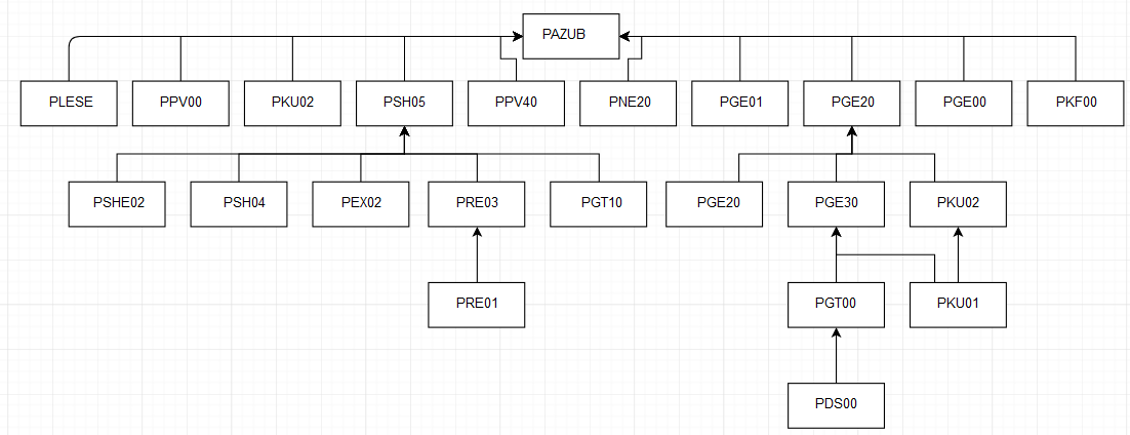
\includegraphics[width=1.25\textwidth]{gfx/Picture/Vorher.PNG}
 \caption{Beispiel der bestehenden Berechtigungsstruktur}
 \label{fig:AltBer}
\hspace*{-2cm}
 \centering
 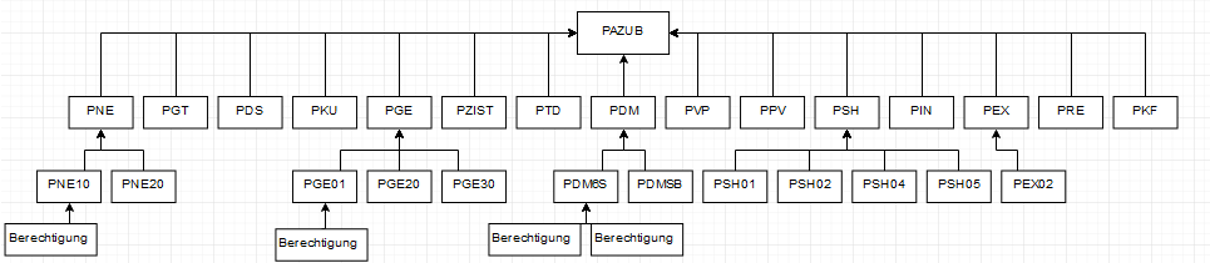
\includegraphics[width=1.25\textwidth]{gfx/Picture/Nachher.PNG}
 \caption{Beispiel der neuen Berechtigungsstruktur}
 \label{fig:NeuBer}
\end{figure}
\newpage
Das Bild (\ref{fig:AltBer}) zeigt eine bestehende Berechtigungsstruktur.
(\ref{fig:AltBer}) hingegen bildet die Struktur nach den neuen Konventionen dar.
Diese beide Bilder wurden denselben IT-Spezialisten gezeigt, die befragt wurden.
Einheitlich haben alle befragten IT-Spezialisten angegeben, dass Sie die neue Struktur übersichtlicher und einfacher zu verstehen ist.
Zudem kann man auch erkennen, dass die Hierarchie verringert wurde.
\newline
Das aktuelle Verfahren, das verwendet wird um die Berechtigung zu überprüfen gleicht einem Insertion-Sort.
Dabei durch jedes einzelne Profil durch gegagen bis die gewünsche Berechtigungen gefunden wurde.
Dies weißt eine Komplexität von n im Optimalfall und $n^2$ im schlimmsten Falle auf.
n beschreibt dabei, die Anzahl von Profilen/Berechtigungen, die der Algorithmus durchlaufen muss. \cite{weblogIn,log} (S. 12)
\newline
Bei der neuen Struktur kann ein Merge-Sort genutzt werden.
Dabei würde der Algorithmus auf bestimmte Eigenschaften der Profile achten.
Würde zum Beispiel verlangt werden, ob der Nutzer eine Berechtigung für PNE10 hat, würde nur der Baum von PNE durchsucht werden und in diesem Falle direkt PNE10 ausgewählt werden.
Dieser Suchalgorithmus ist komplexer als der Insertion-Sort, ist jedoch deutlich effizienter bei einer größeren Menge von Profilen und Berechtigungen.
Dessen Komplexität beläuft n*log(n) im besten sowie im schlechtesten Fall. \cite{weblogMer,log} (S. 12)
\newline
Wenn beispielsweise n = $100$ wäre, würden die Ergebnisse wie folgt aussehen:
\newline
\newline
Best-Case(Insert) = $100$
\newline
Worst-Case(Insert) = $100^2 = 10.000$
\newline
\newline
Best-Case(Merge) = $100*log(100) = 200$
\newline
Worst-Case(Merge) = $100*log(100) = 200$
\newline
\newline
Wie man erkennen kann ist der neue Algorithmus langsamer im Best-Case, aber deutlich schneller im Worst-Case und bietet allgemein eine konsistente Zeit, welche für eine Versicherung wichtig ist.
Der Insertion-Sort sowie der Merge-Sort haben auch eine average Formel: \cite{weblogMer,weblogIn}
\newline
\newline
Average(Insert) = $100^2 = 10.000$
\newline
\newline
Average(Merge) = $100*log(100) = 200$
\newline
\newline
Man kann erkennen, dass im normalen Falle die neue Struktur mit dem Merge-Sort deutlich effektiver ist als die bestehende Struktur.
Diese würde durchschnittlich 50\% effektiver sein.

\section{Konzept Minimalistisch}
\label{sec:chapter04:minimal}
Aliquam ut pretium lectus. Curabitur in eros et sapien aliquet luctus ut sit amet eros. Proin et libero non mi venenatis aliquet at sed lorem. Ut sed enim mi, id viverra eros. Cras metus ante, placerat id commodo at, molestie non libero. Aenean eu risus erat, vel consequat metus. Sed malesuada metus sit amet nisl viverra hendrerit.


